\documentclass{classrep}
\usepackage[utf8]{inputenc}
\frenchspacing

\usepackage{graphicx}
\usepackage[usenames,dvipsnames]{color}
\usepackage[hidelinks]{hyperref}
\usepackage{lmodern}
\usepackage{graphicx}
\usepackage{placeins}
\usepackage{url}
\usepackage{amsmath, amssymb, mathtools}
\usepackage{listings}
\usepackage{fancyhdr, lastpage}
\usepackage{adjustbox}
\usepackage{makecell}

\pagestyle{fancyplain}
\fancyhf{}
\renewcommand{\headrulewidth}{0pt}
\cfoot{\thepage\ / \pageref*{LastPage}}

%--------------------------------------------------------------------------------------%
\studycycle{Informatyka stosowana, studia dzienne, II st.}
\coursesemester{I}

\coursename{Wprowadzenie do Data Science i metod uczenia maszynowego}
\courseyear{2020/2021}

\courseteacher{mgr inż. Rafał Woźniak}
\coursegroup{Wtorek, 13:15}

\author{%
    \studentinfo[239661@edu.p.lodz.pl]{Szymon Gruda}{239661}\\
    \studentinfo[239671@edu.p.lodz.pl]{Jan Karwowski}{239671}\\
    \studentinfo[239673@edu.p.lodz.pl]{Michał Kidawa}{239673}\\
    \studentinfo[239676@edu.p.lodz.pl]{Kamil Kowalewski}{239676}\\
}

\title{Zadanie 5.: Problem Set 5}

\begin{document}
    \maketitle
    \thispagestyle{fancyplain}

    \newpage
    \tableofcontents
    \newpage

    \section{Wprowadzenie}
    \label{intro} {
        Do poniższych zadań klasyfikacji oraz klasteryzacji zostały wykorzystane takie
        same zbiory jak w zadaniu 3 - klasyfikacja oraz zadaniu 4 - klasteryzacja.

        \subsection{Klasyfikacja}
        \label{intro:classification} {
            Do badań zostały wykorzystane następują klasyfikatory z wybranymi
            parametrami.\\
            \textbf{Zbiór Heart:}
            \begin{itemize}
                \item KNN - \textit{k=9}, \textit{metryka=Euclidesowa}
                \item Bayes - brak parametrów
                \item SVM - \textit{kernel=poly}, \textit{C=1.6}, \textit{gamma=0.0001}
                \item Lasy losowe - \textit{min\_samples\_leaf=10}, \textit{n\_estimators=50}, \textit{max\_samples=0.5}
            \end{itemize}
            \

            \textbf{Zbiór Gestures:}
            \begin{itemize}
                \item KNN - \textit{k=9}, \textit{metryka=Euclidesowa}
                \item Bayes - brak parametrów
                \item SVM - \textit{kernel=rbf}, \textit{C=2.0}, \textit{gamma=0.0001}
                \item Lasy losowe - \textit{min\_samples\_leaf=8}, \textit{n\_estimators=500}
            \end{itemize}
            \

            \textbf{Zbiór Weather:}
            \begin{itemize}
                \item KNN - \textit{k=9}, \textit{metryka=Euclidesowa}
                \item Bayes - brak parametrów
                \item SVM - \textit{kernel=rbf}, \textit{C=1.6}, \textit{gamma=0.001}
                \item Lasy losowe - \textit{max\_depth=5}, \textit{n\_estimators=200}, \textit{max\_samples=0.05}
            \end{itemize}
        }

        \subsection{Klasteryzacja}
        \label{intro:clustering} {
            Do badań zostały wykorzystane następujące modele klasteryzacji z wybranymi
            parametrami.\\
            \textbf{Zbiór Iris:}
            \begin{itemize}
                \item K-Means - \textit{k=3}
                \item Metoda aglomeracyjna -  \textit{k=3}, \textit{metryka=Manhattan},
                \textit{linkage=complete}
                \item Metoda expectation-maximization - \textit{k=4},
                \textit{covariance\_type=full},
                \textit{max\_iter=200},
                \item DBSCAN - \textit{min\_samples=7}, \textit{epsilon=0.9}, \textit{metryka=minkowski}
            \end{itemize}
            \

            \textbf{Zbiór Customers:}
            \begin{itemize}
                \item K-Means - \textit{k=6}
                \item Metoda aglomeracyjna -  \textit{k=6}, 
                \textit{linkage=Ward}
                \item Metoda expectation-maximization - \textit{k=6},
                \textit{covariance\_type=diag},
                \textit{max\_iter=200},
                \item DBSCAN - \textit{min\_samples=7}, \textit{epsilon=23}, \textit{metryka=minkowski}
            \end{itemize}
            \

            \textbf{Zbiór Moons:}
            \begin{itemize}
               \item K-Means - \textit{k=8}
                \item Metoda aglomeracyjna -  \textit{k=8},
                \textit{linkage=Ward}
                \item Metoda expectation-maximization - \textit{k=9},
                \textit{covariance\_type=full},
                \textit{max\_iter=200},
                \item DBSCAN - \textit{min\_samples=5}, \textit{epsilon=0.2}, \textit{metryka=minkowski}
            \end{itemize}
        }

    }
    \newpage

    \section{Wyniki}
    \label{results} {

        \subsection{Klasyfikacja}
        \label{results:classification} {

            \subsubsection{Zbiór Heart} {

                \begin{table}[!htbp]
                    \centering
                    \begin{tabular}{|c|c|c|c|c|}
                        \hline
                        Classifier & Accuracy & Sensitivity & Specificity & Precision \\ \hline
                        knn & 0.7143 & 0.7292 & 0.6977 & 0.7292 \\ \hline
                        bayes & 0.8132 & 0.7708 & 0.8605 & 0.8605 \\ \hline
                        svm & 0.8242 & 0.8958 & 0.7442 & 0.7963 \\ \hline
                        random forest & 0.8791 & 0.875 & 0.8837 & 0.8936 \\ \hline
                    \end{tabular}
                    \caption
                    [Heart basic metrics]{}
                    \label{Heart_basic_metrics}
                \end{table}
                \FloatBarrier

                \begin{table}[!htbp]
                    \begin{minipage}{.24\textwidth}
                        \centering
                        \begin{tabular}{|c|c|}
                            \hline
                            30 & 13 \\ \hline
                            13 & 35 \\ \hline
                        \end{tabular}
                        \caption
                        [Heart knn confusion matrix]{knn}
                        \label{Heart_knn_confusion_matrix}
                    \end{minipage}
                    \hfill
                    \begin{minipage}{.24\textwidth}
                        \centering
                        \begin{tabular}{|c|c|}
                            \hline
                            37 & 6 \\ \hline
                            11 & 37 \\ \hline
                        \end{tabular}
                        \caption
                        [Heart bayes confusion matrix]{bayes}
                        \label{Heart_bayes_confusion_matrix}
                    \end{minipage}
                    \hfill
                    \begin{minipage}{.24\textwidth}
                        \centering
                        \begin{tabular}{|c|c|}
                            \hline
                            32 & 11 \\ \hline
                            5 & 43 \\ \hline
                        \end{tabular}
                        \caption
                        [Heart svm confusion matrix]{svm}
                        \label{Heart_svm_confusion_matrix}
                    \end{minipage}
                    \hfill
                    \begin{minipage}{.24\textwidth}
                        \centering
                        \begin{tabular}{|c|c|}
                            \hline
                            38 & 5 \\ \hline
                            6 & 42 \\ \hline
                        \end{tabular}
                        \caption
                        [Heart random forest confusion matrix]{random forest}
                        \label{Heart_random_forest_confusion_matrix}
                    \end{minipage}
                    \caption{Macierze pomyłek}
                \end{table}
                \FloatBarrier

                \begin{figure}[!htbp]
                    \centering
                    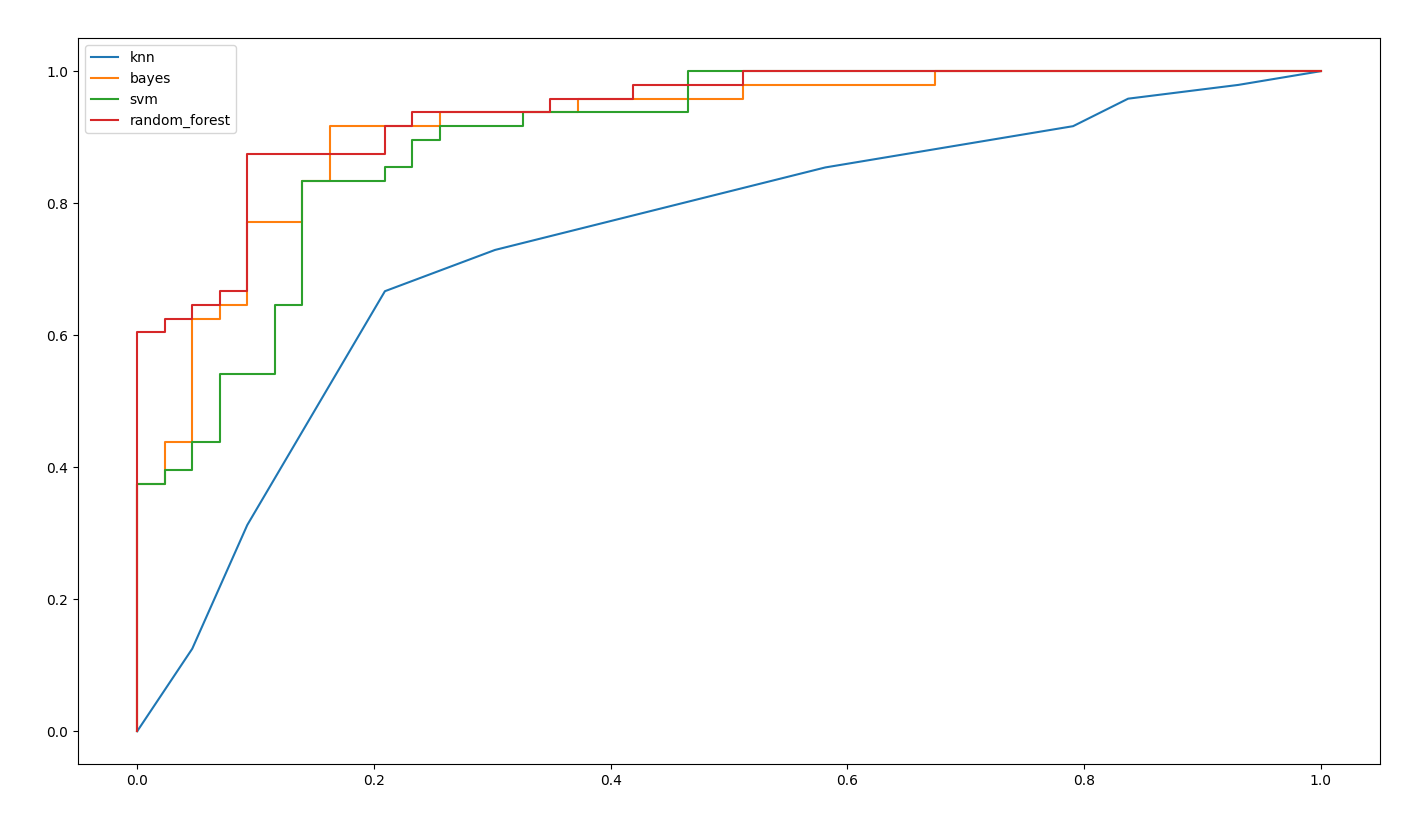
\includegraphics
                    [width=1.2\textwidth,keepaspectratio]
                    {img/heart_roc.png}
                    \caption
                    {Krzywa ROC}
                \end{figure}
                \FloatBarrier

                \begin{figure}[!htbp]
                    \centering
                    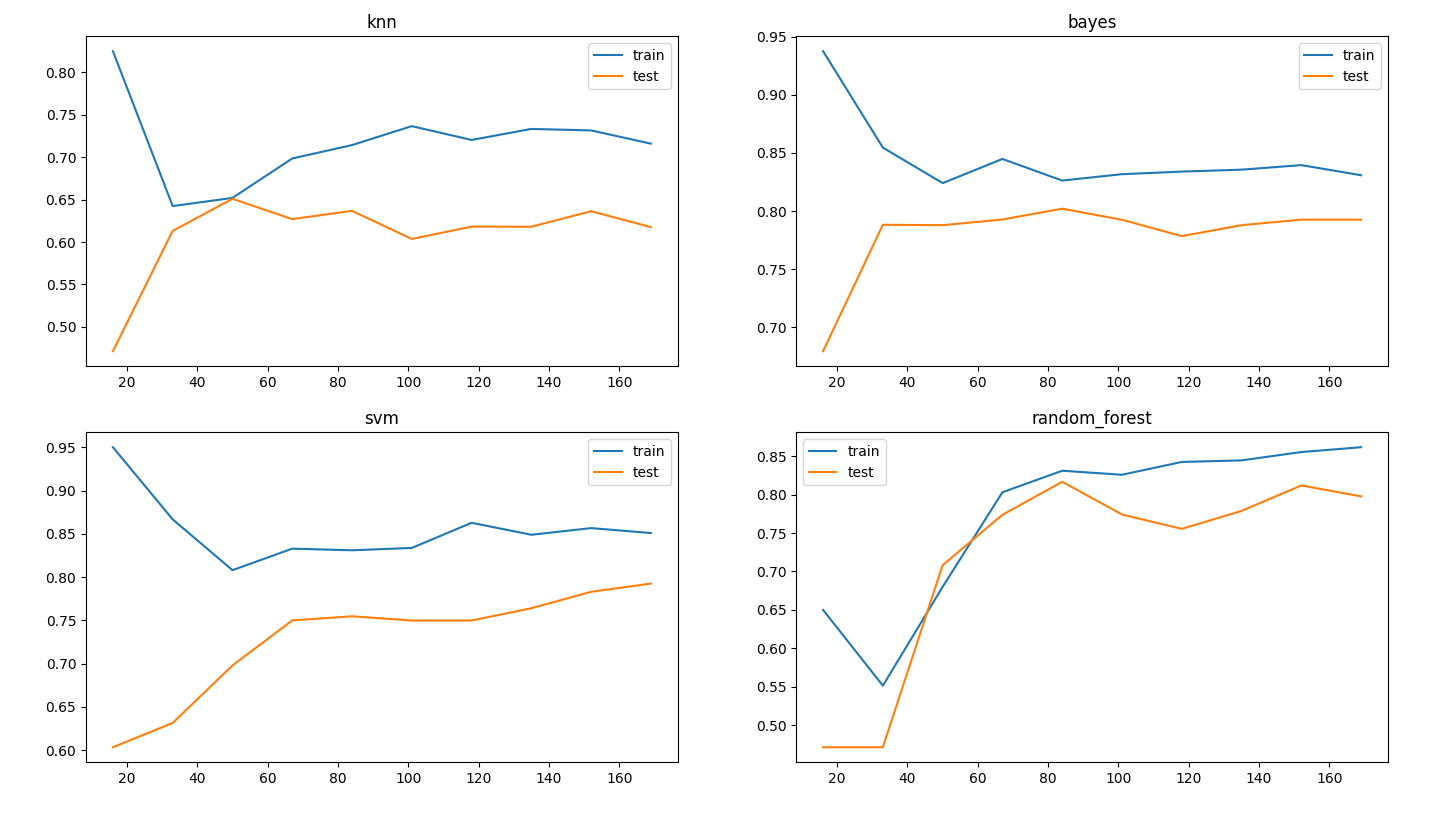
\includegraphics
                    [width=1.18\textwidth,keepaspectratio]
                    {img/heart_learning.png}
                    \caption
                    {Krzywa uczenia}
                \end{figure}
                \FloatBarrier
            }

            \subsubsection{Zbiór Gestures} {

                \begin{table}[!htbp]
                    \centering
                    \begin{tabular}{|c|c|c|c|}
                        \hline
                        Classifier & Accuracy & Sensitivities & Precisions \\ \hline
                        knn & 0.6821 & [0.8708 0.9374 0.1254 0.7758] & [0.9949 0.5744 0.8926 0.5845] \\ \hline
                        bayes & 0.8779 & [0.9157 0.9451 0.9048 0.7378] & [0.924  0.8206 0.9431 0.8316] \\ \hline
                        svm & 0.8913 & [0.9674 0.9681 0.7793 0.8422] & [0.9535 0.8819 0.9129 0.8189] \\ \hline
                        random forest & 0.9118 & [0.9551 0.9    0.9373 0.8529] & [0.9169 0.9457 0.9129 0.8694] \\ \hline
                    \end{tabular}
                    \caption
                    [Gestures basic metrics]{}
                    \label{Gestures_basic_metrics}
                \end{table}
                \FloatBarrier

                \begin{table}[!htbp]
                    \begin{minipage}{.48\textwidth}
                        \centering
                        \begin{tabular}{|c|c|c|c|}
                            \hline
                            775 & 74 & 9 & 32 \\ \hline
                            0 & 853 & 0 & 57 \\ \hline
                            3 & 374 & 108 & 376 \\ \hline
                            1 & 184 & 4 & 654 \\ \hline
                        \end{tabular}
                        \caption
                        [Gestures knn confusion matrix]{knn}
                        \label{Gestures_knn_confusion_matrix}
                    \end{minipage}
                    \hfill
                    \begin{minipage}{.48\textwidth}
                        \centering
                        \begin{tabular}{|c|c|c|c|}
                            \hline
                            815 & 1 & 8 & 66 \\ \hline
                            0 & 860 & 28 & 22 \\ \hline
                            15 & 29 & 779 & 38 \\ \hline
                            52 & 158 & 11 & 622 \\ \hline
                        \end{tabular}
                        \caption
                        [Gestures bayes confusion matrix]{bayes}
                        \label{Gestures_bayes_confusion_matrix}
                    \end{minipage}
                \end{table}
                \FloatBarrier

                \begin{table}[!htbp]
                    \begin{minipage}{.48\textwidth}
                        \centering
                        \begin{tabular}{|c|c|c|c|}
                            \hline
                            861 & 15 & 14 & 0 \\ \hline
                            5 & 881 & 4 & 20 \\ \hline
                            11 & 42 & 671 & 137 \\ \hline
                            26 & 61 & 46 & 710 \\ \hline
                        \end{tabular}
                        \caption
                        [Gestures svm confusion matrix]{svm}
                        \label{Gestures_svm_confusion_matrix}
                    \end{minipage}
                    \hfill
                    \begin{minipage}{.48\textwidth}
                        \centering
                        \begin{tabular}{|c|c|c|c|}
                            \hline
                            850 & 0 & 12 & 28 \\ \hline
                            0 & 819 & 37 & 54 \\ \hline
                            14 & 14 & 807 & 26 \\ \hline
                            63 & 33 & 28 & 719 \\ \hline
                        \end{tabular}
                        \caption
                        [Gestures random forest confusion matrix]{random forest}
                        \label{Gestures_random_forest_confusion_matrix}
                    \end{minipage}
                    \caption{Macierze pomyłek}
                \end{table}
                \FloatBarrier

                \begin{figure}[!htbp]
                    \centering
                    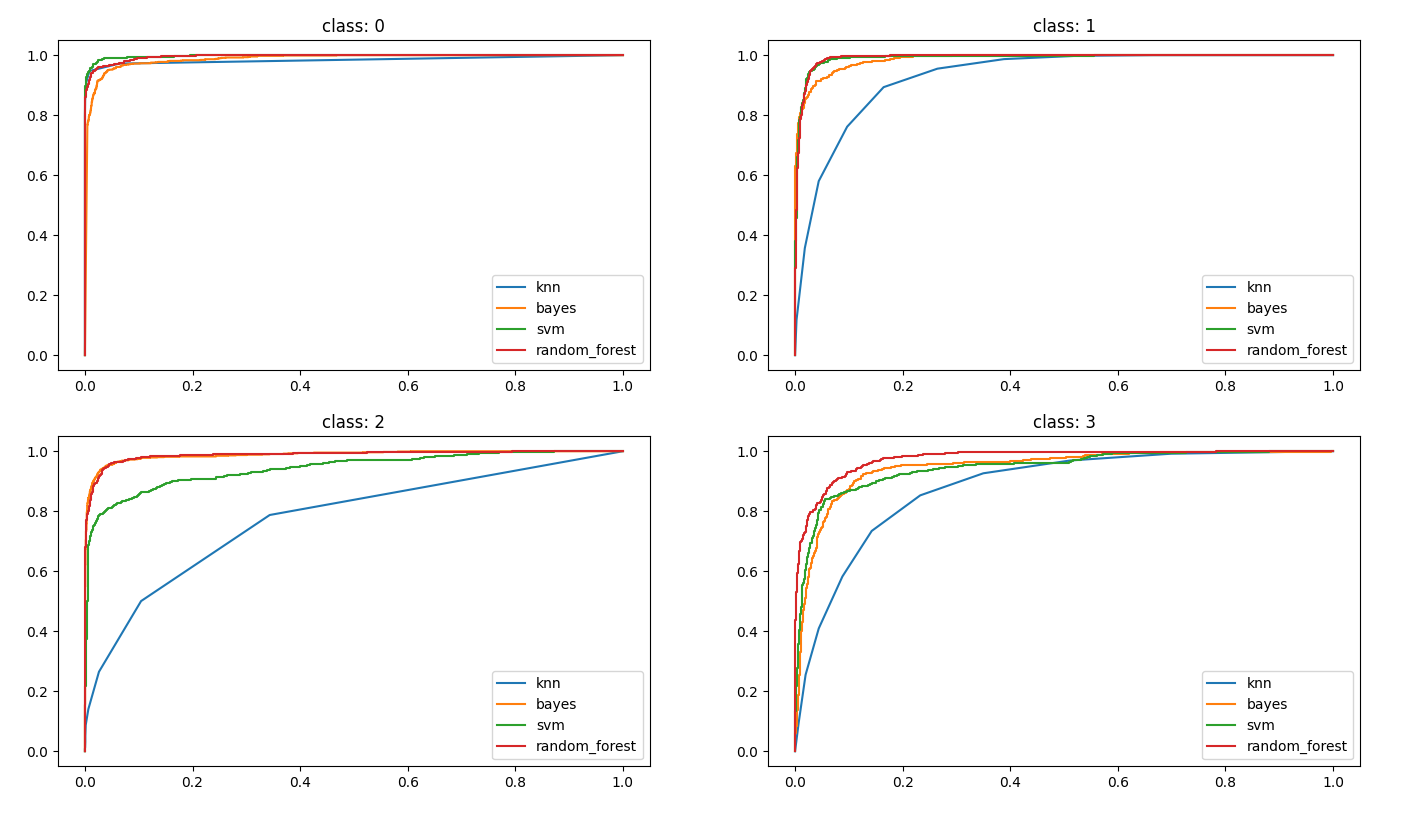
\includegraphics
                    [width=1.2\textwidth,keepaspectratio]
                    {img/gestures_roc.png}
                    \caption
                    {Krzywa ROC}
                \end{figure}
                \FloatBarrier

                \begin{figure}[!htbp]
                    \centering
                    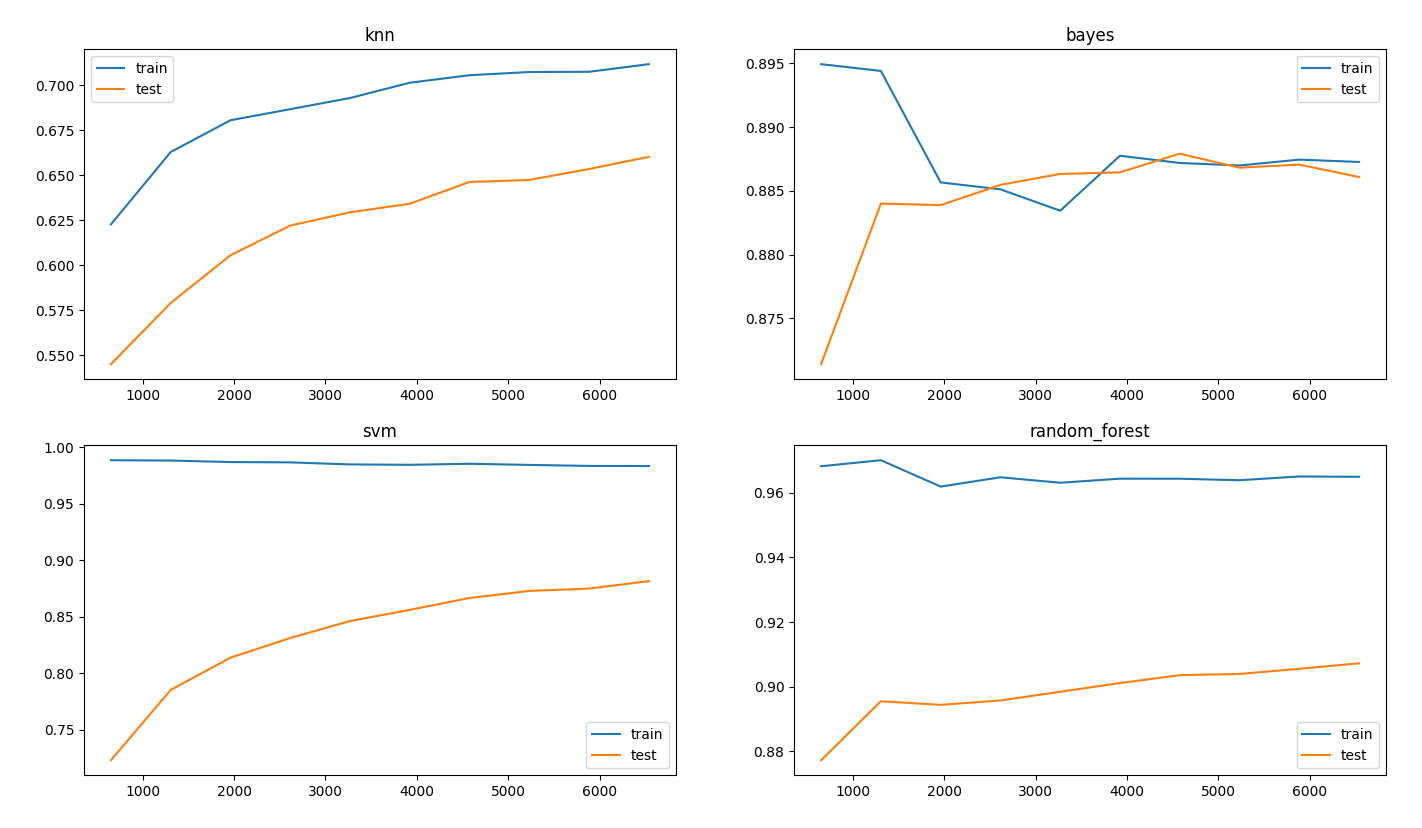
\includegraphics
                    [width=1.2\textwidth,keepaspectratio]
                    {img/gestures_learning.png}
                    \caption
                    {Krzywa uczenia}
                \end{figure}
                \FloatBarrier
            }

            \subsubsection{Zbiór Weather} {

                \begin{table}[!htbp]
                    \centering
                    \begin{tabular}{|c|c|c|c|c|}
                        \hline
                        Classifier & Accuracy & Sensitivity & Specificity & Precision \\ \hline
                        knn & 0.849 & 0.4936 & 0.9505 & 0.74 \\ \hline
                        bayes & 0.8004 & 0.6822 & 0.8342 & 0.5402 \\ \hline
                        svm & 0.8604 & 0.5346 & 0.9534 & 0.7663 \\ \hline
                        random forest & 0.85 & 0.4367 & 0.968 & 0.7959 \\ \hline
                    \end{tabular}
                    \caption
                    [Weather basic metrics]{Weather basic metrics}
                    \label{Weather_basic_metrics}
                \end{table}
                \FloatBarrier

                \begin{table}[!htbp]
                    \begin{minipage}{.24\textwidth}
                        \centering
                        \begin{tabular}{|c|c|}
                            \hline
                            12514 & 652 \\ \hline
                            1904 & 1856 \\ \hline
                        \end{tabular}
                        \caption
                        [Weather knn confusion matrix]{knn}
                        \label{Weather_knn_confusion_matrix}
                    \end{minipage}
                    \hfill
                    \begin{minipage}{.24\textwidth}
                        \centering
                        \begin{tabular}{|c|c|}
                            \hline
                            10983 & 2183 \\ \hline
                            1195 & 2565 \\ \hline
                        \end{tabular}
                        \caption
                        [Weather bayes confusion matrix]{bayes}
                        \label{Weather_bayes_confusion_matrix}
                    \end{minipage}
                    \hfill
                    \begin{minipage}{.24\textwidth}
                        \centering
                        \begin{tabular}{|c|c|}
                            \hline
                            12553 & 613 \\ \hline
                            1750 & 2010 \\ \hline
                        \end{tabular}
                        \caption
                        [Weather svm confusion matrix]{svm}
                        \label{Weather_svm_confusion_matrix}
                    \end{minipage}
                    \hfill
                    \begin{minipage}{.24\textwidth}
                        \centering
                        \begin{tabular}{|c|c|}
                            \hline
                            12745 & 421 \\ \hline
                            2118 & 1642 \\ \hline
                        \end{tabular}
                        \caption
                        [Weather random forest confusion matrix]{random forest}
                        \label{Weather_random_forest_confusion_matrix}
                    \end{minipage}
                    \caption{Macierze pomyłek}
                \end{table}
                \FloatBarrier

                \begin{figure}[!htbp]
                    \centering
                    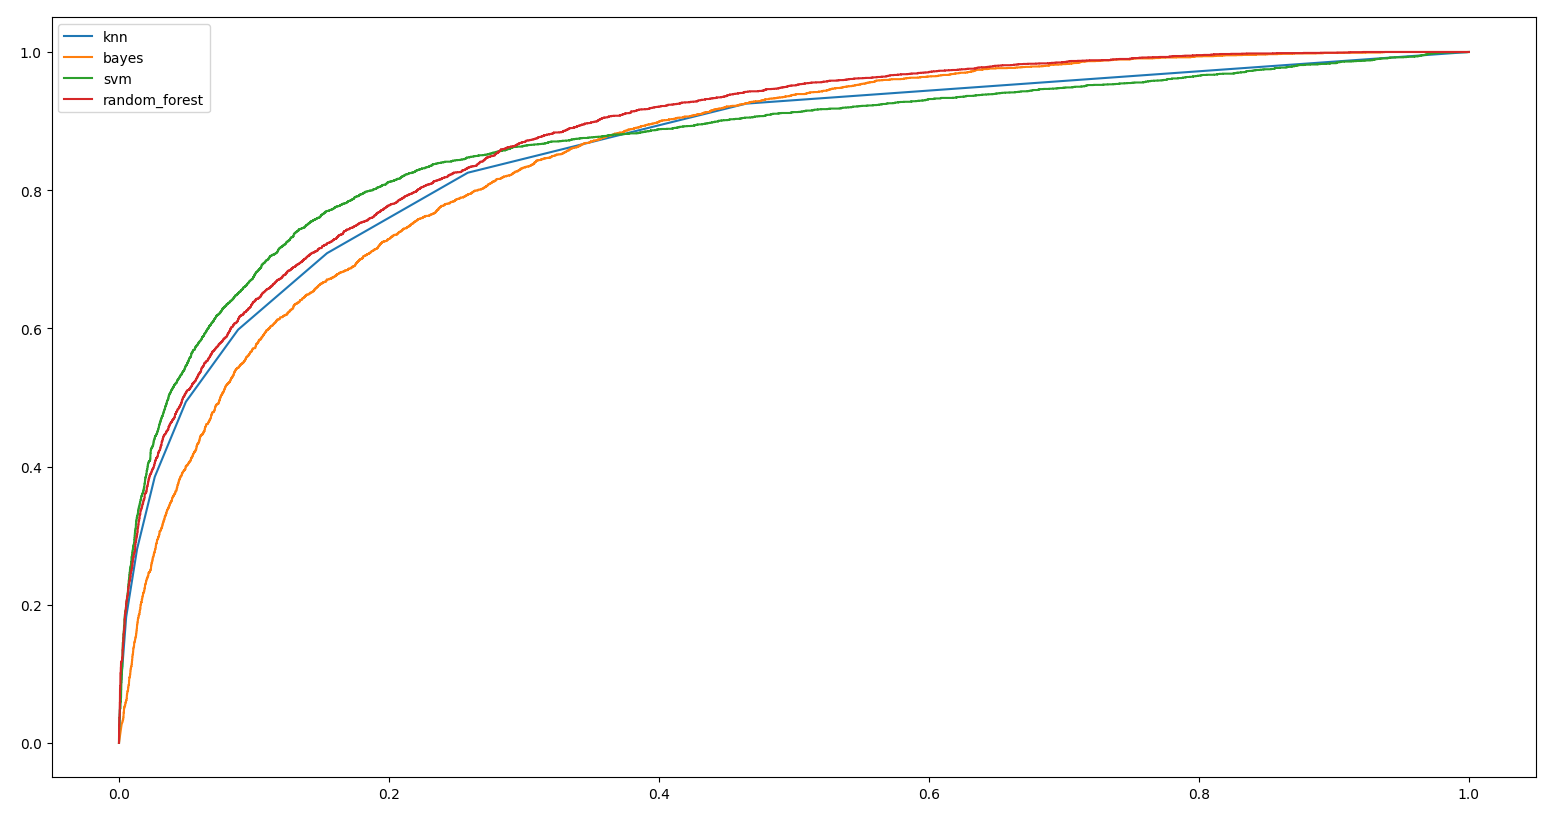
\includegraphics
                    [width=1.2\textwidth,keepaspectratio]
                    {img/weather_roc.png}
                    \caption
                    {Krzywa ROC}
                \end{figure}
                \FloatBarrier

                \begin{figure}[!htbp]
                    \centering
                    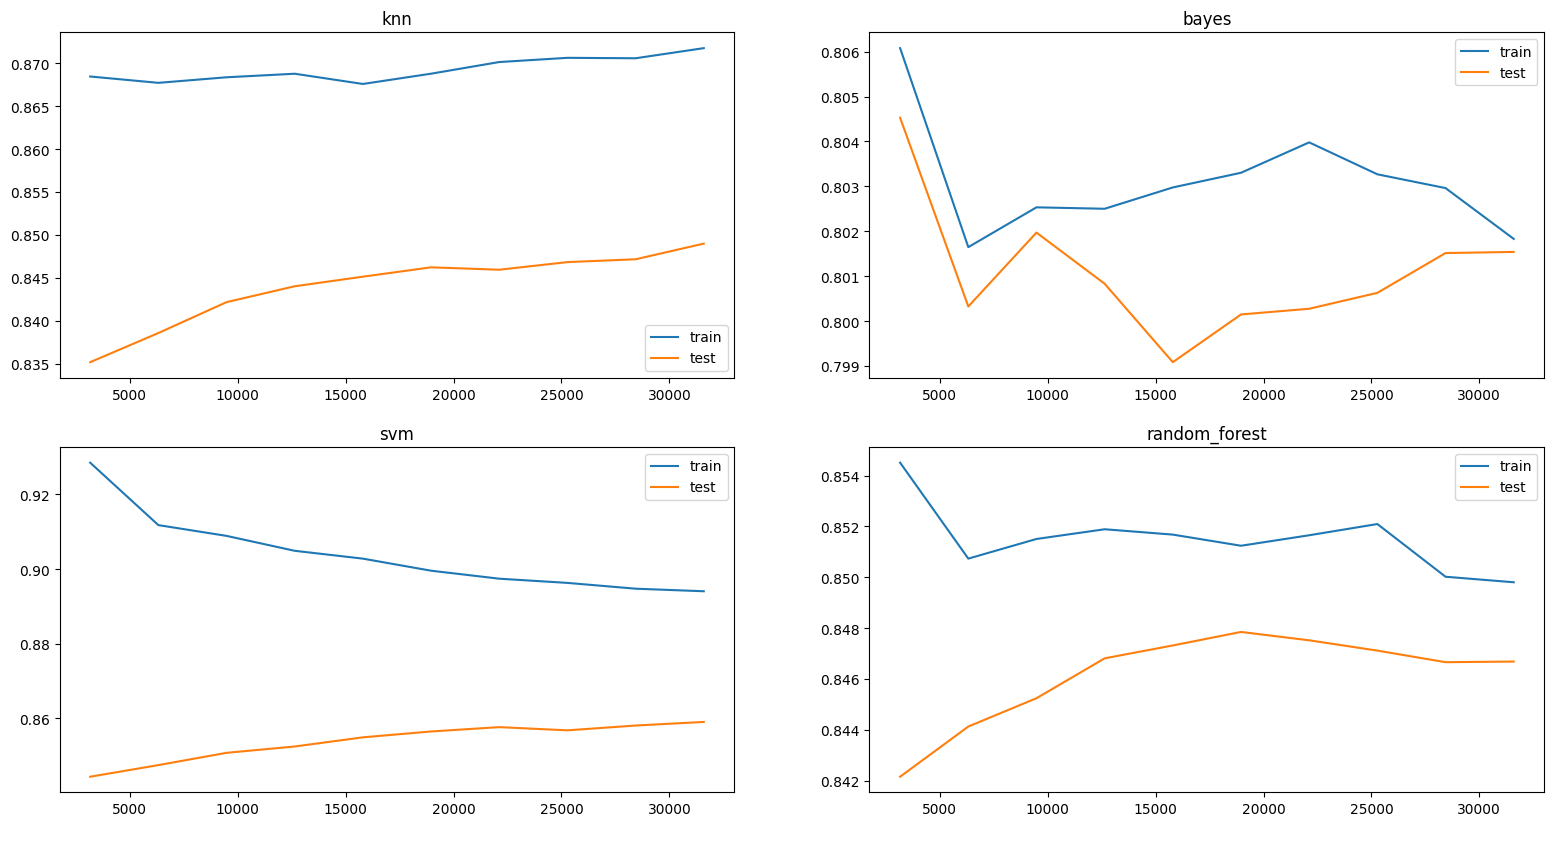
\includegraphics
                    [width=1.2\textwidth,keepaspectratio]
                    {img/weather_learning.png}
                    \caption
                    {Krzywa uczenia}
                \end{figure}
                \FloatBarrier
            }
        }

        \subsection{Klasteryzacja}
        \label{results:clustering} {
            \begin{table}[!htbp]
            \begin{adjustbox}{minipage=20cm, center}
            \centering
            \begin{tabular}{|c|c|c|c|c|c|}
            \hline
            Classifier & Silhouette & Calinski\_Harabasz & Davies\_Bouldin & Rand\_score & Fowlkes\_Mallows \\ \hline
            k\_means & 0.553 & 560.4 & 0.662 & 0.88 & 0.821 \\ \hline
            agglomerative & 0.554 & 551.057 & 0.654 & 0.88 & 0.824 \\ \hline
            \makecell{ expectation\\maximization} & 0.409 & 399.935 & 0.953 & 0.917 & 0.866 \\ \hline
            db\_scan & 0.686 & 501.925 & 0.384 & 0.776 & 0.771 \\ \hline
            \end{tabular}
            \caption
            [Iris basic metrics]{Wyniki wybranych metryk dla zbioru danych Iris}
            \label{Iris_basic_metrics}
            \end{adjustbox}
            \end{table}
            \FloatBarrier
    
            \begin{table}[!htbp]
            \centering
            \begin{tabular}{|c|c|c|c|}
            \hline
            Classifier & Silhouette & Calinski\_Harabasz & Davies\_Bouldin \\ \hline
            k\_means & 0.452 & 166.576 & 0.745 \\ \hline
            agglomerative & 0.443 & 159.329 & 0.769 \\ \hline
            expectation\_maximization & 0.446 & 163.052 & 0.739 \\ \hline
            db\_scan & 0.39 & 4.613 & 0.42 \\ \hline
            \end{tabular}
            \caption
            [Customers basic metrics]{Wyniki wybranych metryk dla zbioru danych Customers}
            \label{Customers_basic_metrics}
            \end{table}
            \FloatBarrier
            
            \begin{table}[!htbp]
            \begin{adjustbox}{minipage=20cm, center}
            \centering
            \begin{tabular}{|c|c|c|c|c|c|}
            \hline
            Classifier & Silhouette & Calinski\_Harabasz & Davies\_Bouldin & Rand\_score & Fowlkes\_Mallows \\ \hline
            k\_means & 0.512 & 1617.388 & 0.583 & 0.622 & 0.493 \\ \hline
            agglomerative & 0.503 & 1517.307 & 0.573 & 0.627 & 0.504 \\ \hline
            \makecell{ expectation\\maximization} & 0.498 & 1630.128 & 0.585 & 0.614 & 0.476 \\ \hline
            db\_scan & 0.325 & 456.067 & 1.16 & 1.0 & 1.0 \\ \hline
            \end{tabular}
            \caption
            [Moons basic metrics]{Wyniki wybranych metryk dla zbioru danych Moons}
            \label{Moons_basic_metrics}
            \end{adjustbox}
            \end{table}
            \FloatBarrier
        }

    }

    \section{Dyskusja}
    \label{summary} {

        \subsection{Klasyfikacja}
        \label{summary:classification} {

            \paragraph{Algorytm K Najbliższych Sąsiadów} sprawuje się zdecydowanie
            gorzej od pozostałych. Widać to bardzo wyraźnie, w przypadku zbiorów danych
            ,,hearts'' oraz ,,gestures'' oraz trochę mniej wyraźnie w przypadku zbioru
            danych ,,weather''. Zaczynając od pierwszego z nich, już po macierzy
            pomyłek można łatwo spostrzec słabość tego algorytmu. Widać też, że zarówno
            sensitivity, specificity jak i precision są niższe niż dla pozostałych
            algorytmów, samo accuracy również. Na wykresie krzywych ROC niebieska linia
            jest znacznie niżej od pozostałych. W przypadku drugiego zbioru danych
            sytuacja jest bardzo podobna - wartości wszystkich metryk są zdecydowanie
            niższe. Ponadto można dostrzec, że klasyfikator w ogóle nie nauczył się
            rozpoznawać przykładów z klasy trzeciej i ma tendencję do
            przyporzadkowywania przykładów do klasy drugiej. Jest zdecydowanie
            niedouczony, co widać dla tego zbioru również po krzywej uczenia. Również
            krzywe ROC prezentują jego niższość, wobec pozostałych metod. Jeżeli chodzi
            o trzeci zbiór danych, to tutaj wszystkie cztery krzywe ROC niemalże się
            pokrywają. Klasyfikatory sprawują się więc stosunkowo podobnie. Można
            jednak zaryzykować stwierdzenie, że KNN podjął tutaj słaby kompromis między
            sensitivity a specificity. To pierwsze ma bardzo niską wartość, a to drugie
            bardzo wysoką. Jego wyniki są najbardziej podobne do działania lasu
            losowego, wykazującego się podobną tendencją, dla zbioru ,,weather''.
            Klasyfikator KNN ma jeszcze tę cechę, że prawie zawsze, więcej przykładów
            uczących mu pomaga osiągnąć lepsze wyniki, zarówno na zbiorze uczącym jak i
            testowym - rosnące krzywe uczenia.

            \paragraph{Naiwny Klasyfikator Bayesa} najbardziej różni się od pozostałych
            algorytmów krzywymi uczenia. Są one najbardziej chaotyczne i zbiegają się,
            a czasem nawet przecinają. W przypadku zbioru danych ,,weather'' są to
            ruchy prawie zupełnie losowe, gdyż zakres na osi dokładności jest bardzo
            niewielki. W przypadku pozostałych zbiorów, wyniki dla zbioru testowego
            przy małej ilości próbek są wyższe, niż dla innych metod. Klasyfikator ten
            ma mniejszą tendencję do przetrenowania i szybciej się uczy. Często
            niewiele daje mu więcej próbek uczących. Jego krzywe ROC są zbliżone do
            krzywych lasu losowego i SVM (poza ostatnim zbiorem danych, gdzie wszystkie
            są podobne). Trudno porównać jego dokładność z pozostałymi algorytmami. Te
            trzy, poza KNN, sprawdzają się bardzo podobnie i jedne osiągają wyższą
            czułość dla jednych klas, a drugie dla innych. Tutaj należałoby stwierdzić,
            co jest właściwym zadaniem klasyfikatora i czy powinien on bardziej skupiać
            się na eliminowaniu błędów pierwszego, czy drugiego rodzaju.

            \paragraph{Maszyna Wektorów Nośnych} sprawuje się podobnie jak Naiwny
            Klasyfikator Bayesa i Lasy Losowe. Charakteryzuje się natomiast tym, że
            trochę podobnie jak w przypadku KNN, zdecydowanie więcej przykładów
            uczących poprawia wyniki na zbiorze testowym. Nie zawsze dzieje się tak
            natomiast w przypadku Naiwnego Klasyfikatora Bayesa i Lasów Losowych. Co do
            ciekawszych spostrzeżeń, to widać również, że dla zbioru ,,weather'' udaje
            się klasyfikatorowi SVM osiągnąć chyba najlepszy kompromis między czułością
            a specyficznością. Krzywa ROC jest najbardziej zbliżona do lewego, górnego
            rogu. W przypadku zbioru ,,gestures'' jest ona natomiast, dla niektórych
            klas, gorsza niż pozostałe algorytmy, a dla innych lepsza, chociaż
            oczywiście zawsze lepsza, niż KNN. Być może wynika to z faktu, że algorytm
            ten jest przystosowany do klasyfikacji binarnej. Poza tymi uwagami,
            sprawuje się on, jak już wspomniano, bardzo podobnie do pozostałych dwóch
            lepszych algorytmów - kwestia zdefiniowania, co jest najbardziej istotne w
            danym zadaniu klasyfikacji.

            \paragraph{Algorytm Lasów Losowych} jest ostatnim i jednocześnie
            prawdopodobnie najlepszym algorytmem klasyfikacji, spośród testowanych w
            ramach tego zadania. Osiąga on najwyższe wartości dokładności, a krzywe ROC
            okazują się być tak samo dobre albo lepsze, niż dla pozostałych algorytmów.
            Dla zbioru ,,hearts'' sprawuje się on zdecydowanie lepiej niż Naiwny
            Klasyfikator Bayesa i bardzo podobnie do SVM (zależy od tego, co w danym
            zadaniu jest krytyczne). Dla zbioru ,,gestures'' również osiąga średnio
            najlepsze wyniki. Tutaj jednak dla różnych klas, różnie sprawują się różne
            klasyfikatory. Można jednak również zaryzykować stwierdzenie, że sprawdził
            się najlepiej - zwłaszcza, że w przypadku wielu klas znacznie trudniej
            wydzielić te bardziej istotne i uśredniony wynik (czyli miara accuracy)
            może okazać się najlepszy do porównania z innymi metodami. W zbiorze ,,
            weather'' osiągnął on dokładność mniejszą niż SVM, który tutaj sprawuje się
            najlepiej. Co więcej, podobnie jak KNN mamy tutaj do czynienia z dużym
            naciskiem na jedną z dwóch klas. Tak więc klasyfikator ten nauczył się
            stosunkowo dobrze rozpoznawać klasę negatywną, natomiast próbki z klasy
            pozytywnej zostały zaklasyfikowane w mniej niż 50\%. Pozwoliło to jednak
            osiągnąć najwyższą precyzję, ze wszystkich klasyfikatorów. Wracamy więc
            znowu do stwierdzenia, że najważniejsze to określić, które miary są
            krytyczne i najistotniejsze - to natomiast zależy od samego tematu -
            dziedziny badań.
        }

        \subsection{Klasteryzacja}
        \label{summary:clustering} {
            Podczas przeprowadzonych eksperymentów badaliśmy wyniki uzyskane przez algorytmy w postaci następujących metryk:
            \begin{itemize}
                \item wewnętrznych: \begin{itemize}
                    \item indeks Silhouette
                    \item indeks Calińskiego-Harabasza
                    \item indeks Daviesa-Bouldina
                \end{itemize}
                \item zewnętrznych: \begin{itemize}
                    \item indeks Rand
                    \item indeks Fowlkes–Mallows
                \end{itemize}
            \end{itemize}

            Ze względu na charakterystykę zbioru Customers (nie ma informacji o
            klasach, które mogą zostać przypisane), niemożliwe było wykorzystanie dla
            niego metryk zewnętrznych. W przypadku każdej z nich poza indeksem
            Daviesa-Bouldina, wyższa wartość oznacza lepszy wynik. Nie można jednak
            porównywać metryk bezpośrednio między sobą.

            W przypadku metryki Silhouette określane jest podobieństwo obiektu do
            własnego skupienia w porównaniu do innych skupień. Indeks przyjmuje
            wartości z przedziału od -1 do +1, gdzie wysoka wartość wskazuje, że dany
            obiekt został dobrze dopasowany do własnego klastra i słabo dopasowany do
            sąsiednich skupień. Najlepsze wartości Silhouette score zostały osiągnięte
            dla metody k-średnich i algorytmu aglomeracyjnego dla zbiorów posiadających
            etykietę. Wartości silhoutte osiągały wyższe wyniki dla metody innej niż
            dbscan z wyjątkiem zbioru danych Irysów, gdzie właśnie dbscan zanotował
            najwyższy wynik, co może być skutkiem samej charakterystyki zbioru.

            Indeks Calinski-Harabasz jest obliczany jako stosunek sumy dyspersji
            pomiędzy klastrami do sumy dyspersji wewnątrz klastra. Dla zbiorów w
            przypadku których analizowane było więcej próbek wartości indeksu osiągały
            większe wartości.

            Davies-Bouldin to indeks, w przypadku którego sprawdzanie poprawności
            grupowania odbywa się przy wykorzystaniu ilości cech charakterystycznych
            dla zestawu danych. Wartości tej metryki osiągały wyższe wyniki dla każdej
            metody poza dbscan z wyjątkiem zbioru danych Moons.

            Indeks Rand oblicza stopień podobieństwa między skupiskami poprzez
            porównanie wszystkich par próbek i obliczenie liczby próbek, które są
            przydzielone poprawnie, lub niepoprawnie do danego skupiska.

            Indeks Fowlkes-Mallows jest obliczany jako wartość średniej geometrycznej
            miar precision oraz recall.
        }

    }

    \section{Wnioski}
    \label{conclusions} {
        \begin{itemize}
            \item Algorytm KNN sprawuje się zazwyczaj gorzej niż inne, bardziej złożone
            algorytmy klasyfikacji, potrzebuje również znacznie więcej przykładów
            uczących. Cechuje go natomiast prostota i łatwość w implementacji.
            \item Pozostałe algorytmy osiągają bardzo zbliżone wyniki, niektóre z
            pozoru mogą wydawać się lepsze od pozostałych poprzez osiągnięcie
            wyższej wartości miary \emph{accuracy}. Po przeanalizowaniu wyników
            innych miar oraz samych macierzy pomyłek, widać wyraźnie, że każdy z
            nich radzi sobie, w jakimś aspekcie, lepiej od pozostałych. Tak więc
            kluczowym dla zadania klasyfikacji jest zdefiniować, która miara jest
            krytyczna - czy bardziej istotne są błędy pierwszego czy drugiego
            rodzaju, a może któraś z wielu różnych klas odgrywa najistotniejszą
            rolę.
            \item Dbscan zadziałał najlepiej w przypadku klasteryzacji zbioru Moons.
            Jako metoda gęstościową najlepiej poradził sobie z danymi zgodnie z
            "intuicją ludzką", co widać po wynikach metryk zewnętrznych
            \item Miary wewnętrzne nie określają jednoznacznie jakości klasyfikacji
        \end{itemize}
    }

    \begin{thebibliography}{0}
        \bibitem{dataset_heart}{https://www.kaggle.com/ronitf/heart-disease-uci}
        \bibitem{dataset_gestures}{https://www.kaggle.com/kyr7plus/emg-4}
        \bibitem{dataset_weather_aus}
        {https://www.kaggle.com/jsphyg/weather-dataset-rattle-package}
        \bibitem{dataset_iris}{https://www.kaggle.com/uciml/iris}
        \bibitem{dataset_customers}
        {https://www.kaggle.com/vjchoudhary7/customer-segmentation-tutorial-in-python}
        \bibitem{dataset_moons}
        {https://scikit-learn.org/stable/modules/generated/sklearn.datasets.make\_moons.html}
    \end{thebibliography}

\end{document}
